\mathchardef\mhyphen="2D

\chapter{Experiments}
\label{chap:experiments}
	\textit{\hspace{0.5cm}This chapter discusses the division of the dataset before training, assessment techniques, and experimental results. Compare the outcomes of the experiments we suggest to the reference experiments from relevant works.}
\minitoc


\section{Classification evaluation metrics}
\label{sec:class_metrics}
\hspace{0.5cm}The effectiveness of a statistical or machine learning\index{Machine learning (ML)} model is assessed using evaluation metrics. These comprise classification accuracy\index{Accuracy}, logarithmic loss, confusion matrix\index{Confusion matrix}, and others. 

It is necessary to analyze the model using a variety of measures. When utilizing one measurement from one assessment metric, a model may perform well, but when using another measurement from another evaluation metric, it may perform poorly. To make sure the model is working properly and ideally, evaluation metrics are essential.

\subsection{Dataset preparation}
\hspace{0.5cm}Splitting is a technique for evaluating the performance of a machine learning algorithm. Train-test split and train-validation-test split are two common types of split.

In the train-test split technique, a dataset is split into two subsets.
The training dataset is the first subset, used to fit the model. Instead of using the second subset to train the model, the input element of the dataset is given to the model, and predictions are then made and compared to the expected values. The testing dataset is the second dataset.
\begin{itemize}
	\item \textbf{Training dataset.} It is used to fit the machine learning model.
	\item \textbf{Testing dataset.} It is used to evaluate the fit machine learning model.
\end{itemize}

The goal is to gauge how well the machine learning model performs on new data, i.e., data not used to train the model. We intend to put the model to use in this manner. In other words, to fit it to the data that is currently available with inputs and outputs that are known, and then to forecast outcomes for new cases in the future where we do not yet have the target values or expected outputs.

The validation dataset is a set that is occasionally necessary. It is known as the train-validation-test split approach. The dataset is divided into three subsets: training dataset, validation dataset, and testing dataset.

\begin{itemize}
	\item \textbf{Training data.} The sample of data used to fit the model.
	\item \textbf{Validation dataset.} The sample of data used to provide an unbiased evaluation of a model fit on the training dataset while tuning model hyperparameters.
	\item \textbf{Testing data.} The sample of data used to provide an unbiased evaluation of a final model fit on the training dataset.
\end{itemize}

\subsection{Confusion matrix}
\hspace{0.5cm}The confusion matrix (error matrix), a tabular depiction of the model predictions versus the ground-truth labels, is one of the fundamental ideas in classification performance. The examples in a predicted class are represented in each row of the confusion matrix\index{Confusion matrix}, while the occurrences in an actual class are represented in each column.  A confusion matrix is
displayed in Table 7.1.

\begin{table}[h!]
	\begin{tabular}{llll}
													   &                            & \multicolumn{2}{c}{Actual class}                                                 \\ \cline{3-4} 
													   & \multicolumn{1}{l|}{}      & \multicolumn{1}{l|}{\textbf{TRUE}}                & \multicolumn{1}{l|}{\textbf{FALSE}}               \\ \cline{2-4} 
	\multicolumn{1}{c|}{\multirow{2}{*}{Predicted class}} & \multicolumn{1}{l|}{\textbf{TRUE}}  & \multicolumn{1}{l|}{True Positive (TP)}  & \multicolumn{1}{l|}{False Positive (FP)} \\ \cline{2-4} 
	\multicolumn{1}{c|}{}                              & \multicolumn{1}{l|}{\textbf{FALSE}} & \multicolumn{1}{l|}{False Negative (FN)} & \multicolumn{1}{l|}{True Negative (TN)}  \\ \cline{2-4} 
	\end{tabular}
	\caption{\label{demo-table} Confusion matrix}
\end{table} 

As we can see diagonal elements of this matrix denote the correct prediction for different classes, while the off-diagonal elements denote the samples which are misclassified.
The confusion matrix can be normalized to obtain the rates. The normalized confusion matrix is presented in Table 7.2. Instead of TP, FN, FP\index{False positive}, TN, normalized confusion matrix uses True Positive Rate (TPR), False Negative Rate (FNR), False Positive Rate (FPR), True Negative Rate (TNR). The most important figures here are FPR (also called false alarm rate) and FNR (miss detection rate).

\begin{table}[h!]
	\begin{tabular}{llll}
													   &                            & \multicolumn{2}{c}{Actual class}                                                 \\ \cline{3-4} 
													   & \multicolumn{1}{l|}{}      & \multicolumn{1}{l|}{\textbf{TRUE}}                & \multicolumn{1}{l|}{\textbf{FALSE}}               \\ \cline{2-4} 
	\multicolumn{1}{c|}{\multirow{2}{*}{Predicted class}} & \multicolumn{1}{l|}{\textbf{TRUE}}  & \multicolumn{1}{l|}{TPR = TP/(TP+FN)}  & \multicolumn{1}{l|}{FPR = FP/(FP+TN)} \\ \cline{2-4} 
	\multicolumn{1}{c|}{}                              & \multicolumn{1}{l|}{\textbf{FALSE}} & \multicolumn{1}{l|}{FNR = FN/(TP+FN)} & \multicolumn{1}{l|}{TNR = TN/(FP+TN)}  \\ \cline{2-4} 
	\end{tabular}
	\caption{\label{demo-table} Normalized confusion matrix}
\end{table} 

\subsection{Classification accuracy}
\hspace{0.5cm}Classification accuracy\index{Accuracy} is one of the most straightforward metrics one can think of. It is calculated by dividing the proportion of accurate predictions by all possible predictions and multiplying the result by 100. The equation of classification accuracy is.
\begin{align*}
	accuracy = 100\left (\frac{TP + TN}{TP + TN + FN + FP}  \right )
\end{align*}

\subsection{Precision}
\hspace{0.5cm}Classification accuracy sometimes fails to serve as an accurate reflection of model performance. One of these cases is when there is an imbalance in the distribution of the classes, with one class being more prevalent than the others. In this scenario, even if every sample is expected to belong to the most common class, we would still have a high accuracy rate, which is completely illogical given that the model is not learning anything and is simply forecasting every sample to belong to the top class. Therefore we need to look at class-specific performance metrics too, such as precision\index{Precision}, which is defined as.
\begin{align*}
	precision = \frac{TP}{TP + FP}
\end{align*}

\subsection{Recall}
\hspace{0.5cm}Recall\index{Recall} is another important metric, which is defined as the fraction of samples from a class which are correctly predicted by the model. It is shown in following equation.
\begin{align*}
	recall = \frac{TP}{TP + FN}
\end{align*}

\subsection{F1-score}
\hspace{0.5cm}Recall or precision\index{Precision} could be given a higher emphasis depending on the application. However, there are a lot of applications where both recall and precision are crucial. Therefore, it seems sensible to consider how to integrate these two metrics into a single one. The F1-score\index{F1-score}, which is the harmonic mean of precision and recall, is one well-known statistic that combines precision and recall.
\begin{align*}
	\mathit{F1\mhyphen score} = \frac{2 \times precision \times recall}{precision + recall}
\end{align*}

The generalized version of the F1-score is.
\begin{align*}
	F_\beta = \left(1 + \beta^2 \right)\frac{2 \times precision \times recall}{\beta^2 \times precision + recall}
\end{align*}

as we can see F1-score is a special case of $F_\beta$ when $\beta$ = 1.

\section{Machine learning models evaluation}
\label{sec:model_evaluation}

\subsection{Logistic regression validator}
\subsubsection{Criteria and dataset preparation}
\hspace{0.5cm}This module is one of the two validators for the WAF\index{WAF}, so not missing any suspicious requests is our top priority. However, this is only a part of our module, built with the criteria of fast and light, easy to run on many different configurations, so the accuracy\index{Accuracy} may not be as high as other approaches. False positive is another major problem. 

\newpage
\subsubsection{Experimental results}
\hspace{0.5cm}The experimental results of logistic regression\index{Logistic regression} are presented in Figure 7.1.

\begin{figure}[!h]
	\centering
	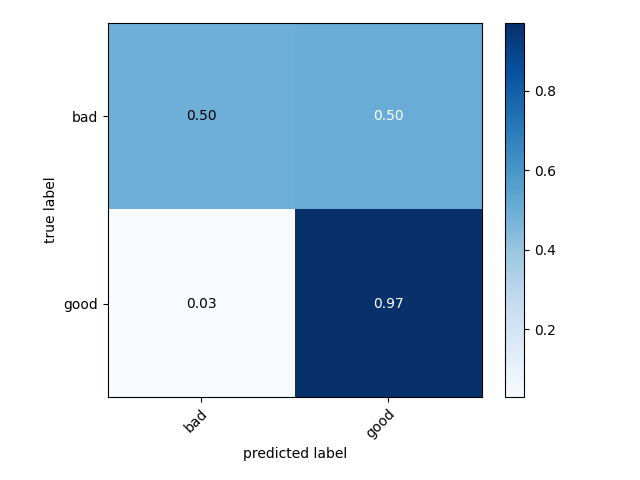
\includegraphics[width=\linewidth, height=10cm,keepaspectratio]{figures/confusion logistic.png}
  \caption{Confusion matrix of logistic regression model}
\end{figure}

The result of the logistic regression model is presented below.
\begin{itemize}
	\item \textbf{Train accuracy:} 88.56\%
	\item \textbf{Test accuracy:} 86,89\%
\end{itemize}

% \begin{table}[h!]
% \centering
% 	\begin{tabular}{l|llll}
% 	\hline
% 				 & \textbf{precision} & \textbf{recall} & \textbf{f1-score} & \textbf{support} \\ \hline
% 	bad          & 0.52      & 0.86   & 0.65     & 1430    \\
% 	good         & 0.97      & 0.87   & 0.92     & 8568    \\
% 				 &           &        &          &         \\
% 	accuracy     &           &        & 0.87     & 9998    \\
% 	macro avg    & 0.75      & 0.87   & 0.78     & 9998    \\
% 	weighted avg & 0.91      & 0.87   & 0.88     & 9998   
% 	\end{tabular}
% 	\caption{\label{demo-table} Logistic regression model evaluation}
% \end{table}

\begin{table}[h!]
	\centering
	\begin{tabular}{l|cccc}
	\hline
				 & \multicolumn{1}{l}{\textbf{Precision}} & \multicolumn{1}{l}{\textbf{Recall}} & \multicolumn{1}{l}{\textbf{F1-score}} & \multicolumn{1}{l}{\textbf{Support}} \\ \hline
	bad          & \textcolor{red}{\textbf{0.52}}                          & 0.86                                & 0.65                                  & 1430                                 \\
	good         & \textcolor{red}{\textbf{0.97}}                          & 0.87                                & 0.92                                  & 8568                                 \\
				 &                                        &                                     &                                       &                                      \\
	accuracy     &                                        &                                     & 0.87                                  & 9998                                 \\
	macro avg    & 0.75                                   & 0.87                                & 0.78                                  & 9998                                 \\
	weighted avg & 0.91                                   & 0.87                                & 0.88                                  & 9998  \\ \hline                              
	\end{tabular}
	\caption{\label{demo-table} Logistic regression model evaluation}
	\end{table}

The model has a very good chance of detecting normal requests with a precision\index{Precision} of 97\%, however, performs poorly in identifying malicious requests. Recall is not advised as a metric for evaluating malicious request detection since FP\index{False positive} is more critical. This problem is not alarming, as we will discuss further in this thesis.

% This model is not the greatest but still can be acceptable as can be seen if we solely focus on its results. However, if we look more closely, we will see that this result has some problems. Let's take a look at the results of the confusion matrix when predicting the test set with the above model. According to the Figure, only 73.46\% of requests are correctly predicted to be attacks by the logistic regression model. Given that the model's accuracy\index{Accuracy} prediction for a normal request is 97.16\%, it is clear that the model will put more emphasis on preventing erroneous preventing of legitimate users than on identifying assaults. This is relatively appropriate because, from the standpoint of an application, the accuracy of 97.16\% is insufficient and may even be considered poor. We may use an example:  Using this approach, there will be more than one request misinterpreted as a large amount of traffic for every 100 legitimate requests (just distinct requests) that reach the WAF\index{WAF} system. If the mentioned WAF system is used to protect a customer's website and even one request is wrongly turned down, it can make the user completely worthless. It will be much worse if customers are accidentally prevented from signing in or making transactions on e-commerce websites. The accuracy required to forecast the ``normal'' class must thus be extremely high (above 99.9\%), but the desired accuracy of predicting the ``attack'' class must be at a tolerable level (about 80\%).

% Attack detection should not be prioritized for another reason: when a hacker targets a web application, they will need to test out a wide range of attack methods, from basic to sophisticated. A model that can warn webmasters to take action to stop more assaults only needs to detect roughly 80\% of inbound attacks.

% We found it to be quite challenging to increase the model's accuracy\index{Accuracy} in this situation when testing it with a variety of various parameters. Our model only achieves a 49.51\% success rate in correctly preventing a malicious request. Maybe in favor of being light and fast, we have to trade off the model's ability to detect an attack.

\subsection{CNN Classifier}
\subsubsection{Criteria and dataset preparation}
\hspace{0.5cm}This module is a classifier for the incoming requests to the module. Then based on the proposed approach in \hyperref[chap:proposed_approaches]{\textbf{Chapter 4}}, the validator will decide whether the request is normal or not. The model must have a low false alarm rate and no miss detection rate. It means the model must achieve almost zero FPR, and zero FNR, which leads to over 95\% precision\index{Precision}, especially in the category \textit{plaintext}. Another vital criterion is time efficiency. A WAF\index{WAF} must respond to block or not to block a request immediately. Therefore the time processing of each request in the model must be less than 10 milliseconds. 
\subsubsection{Experimental results}
\hspace{0.5cm}The CNN\index{CNN} model is trained in 10 epoch with batch size 128. The precision metric and loss of the model during training process is plotted as Figure 7.2.
       
\begin{figure}[!h]
	\centering
	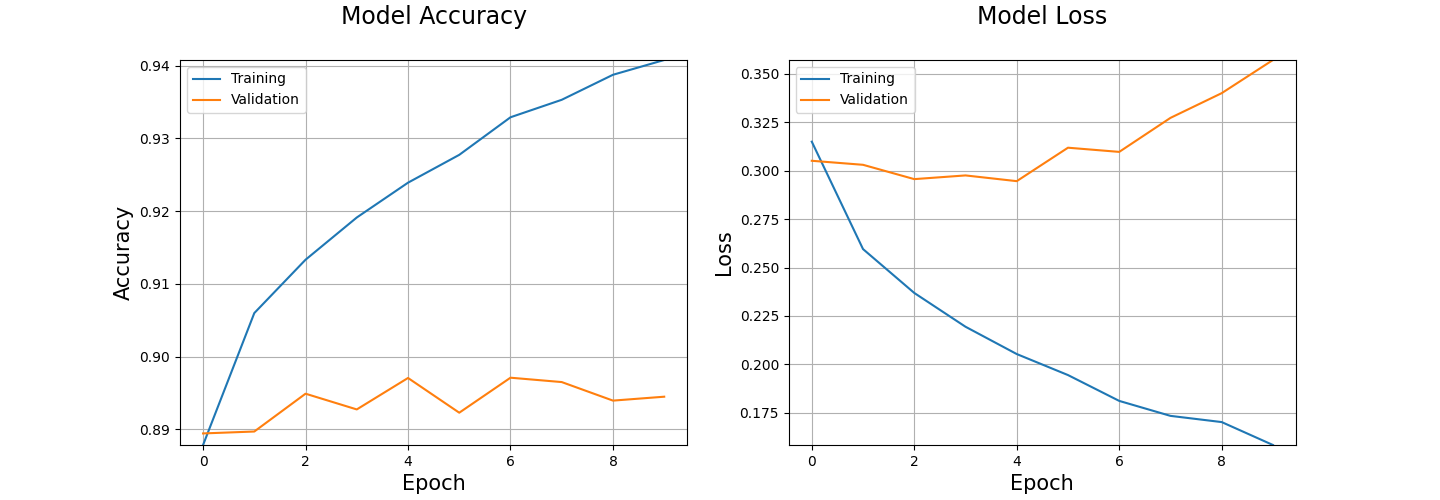
\includegraphics[width=\linewidth, height=10cm,keepaspectratio]{figures/metric and loss.png}
  \caption{The precision metric and loss of the model}  
\end{figure} 

It appears that the model's training set and validation set differ fairly noticeably from one another. The loss of the training dataset decreases continuously, while the loss of the validation set decreases at early steps and starts increasing after a certain point. This demonstrates how ``overfitting'' our model was. The validation loss began below the training loss, then slightly decreased and increased after the fourth epoch. This leads to the stagnation of validation accuracy\index{Accuracy} when the $val\_accuracy$ does not seem to increase. The confusion matrix is displayed in Figure 7.3.

\newpage

\begin{figure}[!h]
	\centering
	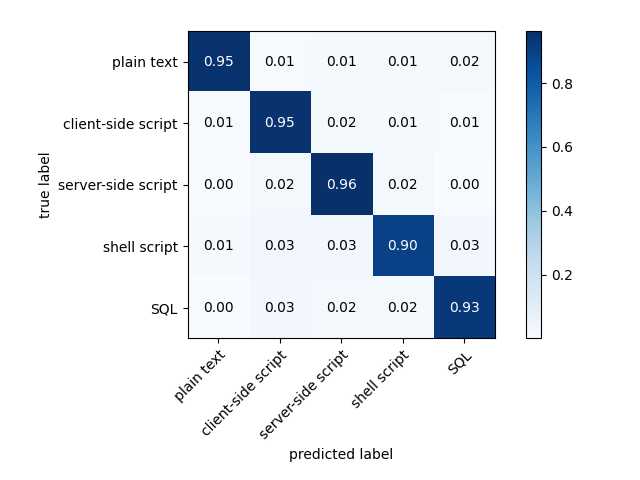
\includegraphics[width=\linewidth, height=10cm,keepaspectratio]{figures/confusion CNN final.png}
  \caption{Structural language classifier model trained}  
\end{figure} 

While the values for other categories are only from 90\% to 95\% correspondingly, it appears that the model has a fair possibility of recognizing regular requests (plain text) with pretty good accuracy\index{Accuracy} and a tiny chance of false alert or miss detection. As the following four categories are all programming languages, it is difficult for the model to separate them, and their weights are lower than plain text (one-fifth). Then the model has succeeded in reducing the blocking of legitimate requests i.e. reducing the false positive rate of WAF\index{WAF}. 
% While the values for other categories are only from 90\% to 95\% correspondingly, it appears that the model has a fair possibility of recognizing regular requests (plain text) with pretty good accuracy and a tiny chance of false alert or miss detection. Because the following four categories are all programming languages, it's difficult for the model to separate them, and their weights are lower than plain text (one-fifth). Then the model succeeded in reducing the blocking of legitimate requests so that it reduced the false positive\index{False positive} rate of WAF\index{WAF}. But in reality, if you look at it from the point of an application, 95\% accuracy is insufficient and even considered inadequate. According to this model, on average, five genuine requests (only separate requests) out of every 100 legitimate requests that pass through the WAF system will be misconstrued for assaults. If the aforementioned WAF system is utilized to defend a customer website and even one request is unintentionally denied, it may render the user useless. If users are mistakenly stopped from signing in or doing transactions on e-commerce websites, the situation will be worse. The accuracy required to forecast the ``normal'' class must therefore be extremely high (above 99.9\%), but the acceptable accuracy of predicting the ``attack'' class must be at a tolerable level (about 80\%). Attack detection should not be prioritized for another reason: when a hacker targets a web application, they are obligated to try out a wide range of attack methods, from basic to complex. A model that can warn administrators to take action to stop more assaults only needs to detect roughly 80\% of incoming attacks.

% In the process of testing the machine learning model with many different parameters, we found it extremely difficult to improve the accuracy of the model in this case. The fact that request data often has a very different standard than normal text, along with the classification of many types of structural languages in our thesis leads to improved accuracy of the model in this case is beyond our ability.

The evaluation metric of the model is presented in Table 7.4.
% \begin{table}[h!]
% \centering
% 	\begin{tabular}{crrrr}
% 	\hline
% 	\textbf{Label}              & \multicolumn{1}{c}{\textbf{Accuracy}} & \multicolumn{1}{c}{\textbf{Precision}} & \multicolumn{1}{c}{\textbf{Recall}} & \multicolumn{1}{c}{\textbf{F1-score}} \\ \hline
% 	\textbf{Plain text}         & 98.56\%                               & 0.95                                   & 0.99                                & 0.97                                  \\
% 	\textbf{Client-side script} & 97.91\%                               & 0.95                                   & 0.95                                & 0.95                                  \\
% 	\textbf{Server-side script} & 97.29\%                               & 0.96                                   & 0.99                                & 0.97                                  \\
% 	\textbf{Shell script}       & 98.4\%                                & 0.90                                   & 0.36                                & 0.52                                  \\
% 	\textbf{SQL}                & 99.34\%                               & 0.93                                   & 0.63                                & 0.75                                  \\ \hline
% 	\end{tabular}
% 	\caption{\label{demo-table} Evaluating the model by precision, recall and F1-score.}
% \end{table}

\begin{table}[h!]
\centering
	\begin{tabular}{lcccc}
	\hline
	\textbf{Label}     & \textbf{Accuracy} & \textbf{Precision} & \textbf{Recall} & \textbf{F1-score} \\ \hline
	Plain text         & \textcolor{red}{\textbf{98.56\%}}  & \textcolor{red}{\textbf{0.95}}      & 0.99            & 0.97              \\
	Client-side script & 97.91\%           & 0.95               & 0.95            & 0.95              \\
	Server-side script & 97.29\%           & 0.96               & 0.99            & 0.97              \\
	Shell script       & 98.4\%            & 0.9                & 0.36            & 0.52              \\
	SQL                & 99.34\%           & 0.93               & 0.63            & 0.75              \\ \hline
	\end{tabular}
	\caption{\label{demo-table} Evaluating the model by precision, recall and F1-score.}
	\end{table}

It is noticeable that the model does not have the best accuracy (only 95.75\% on the test set). However, because there are just two convolutional layers in the model, it processes requests on average in 29ms (with system specifications shown in Table 7.5), meaning that the response is returned nowhere instantly. That time is still acceptable despite not reaching our goal yet (since our model requires the combination of two different models to produce the desired result).

\begin{table}[h!]
\centering
	\begin{tabular}{ll}
	\hline
	\textbf{Hardware} & \textbf{Specification} \\ \hline
	CPU               & Apple M1 (8 cores)     \\
	GPU               & Apple M1 8-core GPU    \\
	RAM               & 16GB                   \\ \hline
	\end{tabular}
	\caption{\label{demo-table} System specifications.}
\end{table}
  
\section{End-to-end experiments}
\hspace{0.5cm}In these experiments, we are considering the default structural language category is plain text, showing that our module is defending an API application (which accepts just plain text queries, i.e. requests in JSON or XML).

We are using CSIC 2020 dataset (\hyperref[subsec:csic_2010]{\textbf{Chapter 6}}) to test our model and compare our work with the related works that also train on the mentioned datasets.

\begin{table}[h!]
\centering
	\begin{tabular}{lll}
	\hline
										  & \textbf{CSIC}       & \textbf{Custom dataset} \\ \hline
	Our propose Logistic Regression model & 86.89\%    & 88.56\%        \\
	Our propose CNN classifier            & Not tested & 94.64\%        \\
	A. Shaheed et al.\cite{Shaheed}                     & 99.59\%    & 98.8\%         \\
	I. Jemal et al. \cite{Jemal}                       & 98.1\%     & Not tested     \\
	M. T. Nguyen et al. \cite{Truong}                      & 99.99\%    & Not tested     \\
	S. Toprak et al. \cite{Toprak}                     & 99.03\%    & Not tested     \\
	D. T. A. M. Devi et al. \cite{Devi}                             & 99.93\%    & Not tested \\ \hline
	\end{tabular}
	\caption{\label{demo-table} Accuracy of our proposed model compared with related works.
	}
\end{table}

We regret to claim that the final stage of our model is currently incomplete. Based solely on what we currently have, it is also clear that in comparison to previous related works, our proposed model has numerous significant flaws.


Based on the result of the two models, we could calculate the probability of the module blocking a request. The module only considers the incoming request as malicious when and only when both of the validators give a negative result
\begin{align*}
	P_{\overline{A}\hspace{0.05cm}\overline{B}} = P_{\overline{A}} \times P_{\overline{B}}.
\end{align*}

With $P_{\overline{A}}$ is the probability that the logistic regression model considers a request as malicious, $P_{\overline{B}}$ is the probability that the CNN\index{CNN} model considers a request as malicious. We have $P_{\overline{A}} = 24.55\%$ and $P_{\overline{B}} = 5\%$, so that the probability that the probability of a request being blocked ($P_{\overline{A}\hspace{0.05cm}\overline{B}}$) is 1.23\%. 

We do not even have to consider the accuracy\index{Accuracy} of the final module. In reality, if you look at it from the standpoint of an application, 1.23\% of blocking the request is insufficient and even considered inadequate. This model predicts that out of every 100 legitimate requests that pass through the WAF\index{WAF} system on average (just distinct requests), over 1 of them will be mistaken for attacks. If the mentioned WAF system is used to defend a customer website and even one request is unintentionally blocked, it may render the user useless. It would be even worse if customers were prevented from logging in or making transactions on e-commerce websites by accident. The accuracy required to forecast the ``normal'' class must therefore be extremely high (above 99.9\%), but the desired accuracy of predicting the ``attack'' class must be at a tolerable level (about 80\%). Attack detection should not be prioritized for another reason: when a hacker targets a web application, he must try out a wide range of attack methods, from basic to complex. A model that can warn administrators to take action to stop more assaults only needs to detect roughly 80\% of incoming attacks. Besides, the response time criterion is also not satisfactory for an effective WAF. 

During the testing phase of the machine learning\index{Machine learning (ML)} model with many different parameters, we found it extremely difficult to improve the accuracy of the model in this case. The fact that request data often has a very different standard than normal text, along with the classification of many types of structural languages in our thesis leads to improving the accuracy of the model in this case is beyond our ability.

% \section{Data preparation} 
% \label{sec:data_preparation}
% 	Đối với các giải thuật học máy nói chung cũng như mạng học sâu nói riêng, việc chuẩn bị dữ liệu là vô cùng quan trọng. Nếu sử dụng mô hình đã huấn luyện để dự đoán trên tập dữ liệu không cùng phân bố với tập dữ liệu được sử dụng để huấn luyện mô hình trước đó thì kết quả dự đoán không thể chính xác. Do đó, phân chia dữ liệu sao cho phân bố trên các tập đồng đều với nhau là một trong những yếu tố quan trọng quyết định tới mức hiệu quả của mạng học sâu. 
	
% 	Sau khi khảo sát các ảnh chụp CT của 20 bệnh nhân, chúng tôi nhận thấy sự xuất hiện các khối u có ảnh đưởng đến phân phối mức sáng của các điểm ảnh trong cơ quan gan. Do đó, chúng tôi chia các bệnh nhân ra 03 nhóm: bệnh nhân không có khối u trong gan, bệnh nhân có một khối u trong gan và bệnh nhân có nhiều khối u trong gan. Chúng tôi chia tập dữ liệu thành ba tập dữ liệu bao gồm tập huấn luyện, tập kiểm thử và tập kiểm tra sao cho mỗi tập đều có bệnh nhân không có u, bệnh nhân có một khối u và bệnh nhân có nhiều khối u. Chi tiết các tập dữ liệu được chúng tôi trình bày trong \autoref{tab:3d_ircadb_01_division}.
% 	\begin{table}[h!]
% 		\centering
% 		\caption{Bảng phân chia các bệnh nhân thành các tập dữ liệu.}
% 		\label{tab:3d_ircadb_01_division}
% 		\begin{tabular}{@{\hspace{4mm}}c@{\hspace{5mm}}ll@{\hspace{9mm}}l@{\hspace{9mm}}lr@{\hspace{5mm}}}
% 			\toprule
% 			\multirow{2}{*}{\textbf{STT}} & \multirow{2}{*}{\textbf{Tập}} & \multicolumn{3}{c}{\textbf{Số lượng khối u gan}} & \multirow{2}{*}{\textbf{\ \ Tổng}} \\ \cmidrule(l){3-5}
% 			&  & \textbf{0 khối u} & \textbf{1 khối u} & \textbf{Nhiều khối u} &  \\ \midrule
% 			1 & Huấn luyện\ \ \ & 5, 7, 11 & 2, 3, 9, 12 & 1, 4, 8, 10, 15, 17, 19 & 14 \\[1mm]
% 			2 & Kiểm thử & 14 & 16 & 6 & 3 \\[1mm]
% 			3 & Kiểm tra & 20 & 18 & 13 & 3 \\ \bottomrule
% 		\end{tabular}
% 	\end{table}

% \section{Evaluation methods} 
% \label{sec:evaluation}
% 	Quá trình đánh giá một mô hình phân đoạn hình ảnh y khoa liên quan đến việc đánh giá độ chính xác của kết quả dự đoán. Hai hoạt động cơ bản cần được tiến hành để đánh giá một cách toàn diện một mô hình là đánh giá định tính và đánh giá định lượng. Đánh giá định lượng cho biết một cách tổng quát độ tốt của mô hình, trong khi đó đánh giá định tính cho biết mức độ ổn định của mô hình trong quá trình làm việc (trong trường hợp xấu nhất, trung bình và tốt nhất). Trong phần này, chúng tôi trình bày 4 độ đo có liên quan bao gồm Precision, Recall, IoU và Dice. Trong đó, IoU và Dice được chúng tôi sử dụng để đánh giá kết quả dự đoán của các mô hình.
% \newpage
% 	Ta quy ước,
% 	\begin{itemize}
% 		\item TP (true positive): số lượng điểm ảnh foreground được dự đoán đúng,
% 		\item TN (true negative): số lượng điểm ảnh background được dự đoán đúng,
% 		\item FP (false positive): số lượng điểm ảnh background bị dự đoán sai,
% 		\item FN (false negative): số lượng điểm ảnh foreground bị dự đoán sai.
% 	\end{itemize}
% 	\begin{description}
% 		\item[Precision] trả lời cho câu hỏi ``Số dự đoán thực sự chính xác chiếm bao nhiêu phần trong số các dự đoán foreground?''. Công thức Precision được định nghĩa trong \autoref{eqn:precision}. Precision càng cao, kết quả dự đoán càng tốt.
% 		\begin{equation}
% 		Precision = \dfrac{TP}{TP + FP} \label{eqn:precision}
% 		\end{equation}
		
% 		\item[Recall] trả lời cho câu hỏi ``Số dự đoán thực sự chính xác chiếm bao nhiêu phần trong số các mẫu foreground''. Công thức Recall được định nghĩa trong \autoref{eqn:recall}. Recall càng cao, kết quả dự đoán càng tốt.
% 		\begin{equation}
% 		Recall = \dfrac{TP}{TP + FN} \label{eqn:recall}
% 		\end{equation}
		
% 		\item[Dice] là độ đo cân bằng giữa Precision và Recall. Trong trường hợp mô hình dự đoán chính xác một lượng nhỏ mẫu thuộc foreground, giá trị Precision sẽ cao, tuy nhiên số lượng false negative sẽ cao theo, nghĩa là giá trị Recall thấp. Trong trường hợp mô hình dự đoán một lượng lớn mẫu thuộc foreground, giá trị Recall sẽ cao, tuy nhiên số lượng false positve sẽ cao theo, tức là giá trị Precision thấp. Dice được tính toán bằng cách sử dụng đồng thời Precision và Recall. Khi giá trị Precision và giá trị Recall cùng cao, giá trị Dice sẽ cao, ngược lại, khi một trong hai giá trị Precision và Recall thấp, giá trị Dice sẽ thấp. Do đó, Dice phù hợp cho các bài toán phân loại có sự mất cân bằng về nhãn. Công thức Dice được định nghĩa trong \autoref{eqn:recall}.
% 		\begin{equation}
% 		Dice = 2 * \dfrac{Precision * Recall}{Precision + Recall}
% 		\end{equation}
% 		\item[IoU\nomenclature{IoU}{Intersection over Union}] cho biết mức độ tương tự giữa hai mẫu $X$ và $Y$. IoU được định nghĩa trong \autoref{eqn:iou}.
% 		\begin{equation}
% 		IoU = \dfrac{|X \cap Y|}{|X| + |Y| - |X \cap Y|} \label{eqn:iou}
% 		\end{equation}
% 	\end{description}

	
% \newpage
% \section{Experiment results} 
% \label{sec:exp_results}
% 	Trước khi tiến hành các thí nghiệm để đánh giá hệ thống, chúng tôi thực hiện kiểm chứng tính hiệu quả của đề xuất cắt giảm độ sâu trong mô hình U-Net, để từ đó chọn ra mô hình tốt hơn phục vụ cho các thí nghiệm về sau. \autoref{tab:dac_ta_sieu_tham_so_thi_nghiem_unet_va_unet_star} đặc tả thông số chi tiết của các thí nghiệm dùng để so sánh tính hiệu quả trước và sau điều chỉnh số tầng ở mô hình U-Net sử dụng convolution 3D.
% 	\begin{table}[h!]
% 		\caption{Thông số các thí nghiệm so sánh tính hiệu quả trước và sau điều chỉnh số tầng ở mô hình U-Net sử dụng convolution 3D.}
% 		\label{tab:dac_ta_sieu_tham_so_thi_nghiem_unet_va_unet_star}
% 		\resizebox{\columnwidth}{!}{
% 			\begin{tabular}{clcllrr}
% 				\toprule
% 				\textbf{STT} & \textbf{Kiến trúc} & \textbf{Số tầng}     & \textbf{BatchNorm\index{Batchnorm}} & \textbf{Hàm lỗi} & \textbf{Learning rate\index{Learning rate}} & \textbf{Momentum}     \\ \midrule
% 				1            & U-Net        & 5 			& Không 			 & CrossEntropy     & 0.0001          		 & 0.90 \\
% 				2            & U-Net*        & 3 					& Không 			 & CrossEntropy     & 0.0001          		 & 0.90 \\
% 				\bottomrule
% 			\end{tabular}
% 		}
% 	\end{table}

% 	\autoref{tab:so_sanh_unet_3_va_5_tang} là kết quả thu được khi so sánh hai mô hình. Từ kết quả này chúng ta thấy rằng, chất lượng phân đoạn hệ thống mạch máu trên tập kiểm tra trước và sau hậu xử lý (cột \textbf{Tập kiểm tra} và \textbf{Tập kiểm tra*}) ở mô hình U-Net* không có nhiều sự khác biệt so với mô hình U-Net. Chứng tỏ, việc cắt giảm hai tầng 4 và 5 trong mô hình U-Net là hợp lý vì chúng không có nhiều đóng góp trong quá trình học. Hơn nữa, việc cắt giảm số tầng giúp cho mô hình trở nên nhẹ hơn, thời gian inference\index{Inference}\footnote{Inference trong lĩnh vực học sâu là thuật ngữ dùng để chỉ giai đoạn mô hình sau huấn luyện được sử dụng để dự đoán các mẫu dữ liệu thử nghiệm. Không giống quá trình huấn luyện, inference không thực hiện lan truyền ngược để tính toán lỗi và cập nhật trọng số.}trung bình cho một tập ảnh CT ở mô hình U-Net* là 4.46 giây, nhanh hơn gần 1 giây so với mô hình U-Net là 5.40 giây. Chênh lệch này tuy nhỏ nhưng sẽ có ý nghĩa rất lớn khi áp dụng mô mình vào thực tiễn với khối lượng dữ liệu khổng lồ. Thời gian dành cho công tác chẩn đoán càng được rút ngắn bao nhiêu, cơ hội chữa trị thành công cho bệnh nhân càng lớn bấy nhiêu. Vì vậy, chúng tôi lựa chọn sử dụng mô hình U-Net* trong các thí nghiệp về sau để đánh giá hệ thống.
% 	\begin{table}[h!]
% 		\caption{Kết quả so sánh tính hiệu quả trước và sau điều chỉnh số tầng ở mô hình U-Net sử dụng convolution 3D.}
% 		\label{tab:so_sanh_unet_3_va_5_tang}
% 		\resizebox{\columnwidth}{!}{
% 			\begin{tabular}{clcccccc}
% 				\toprule
% 				\multicolumn{1}{c}{\multirow{2}{*}{\textbf{\ \ STT\ }}} & \multicolumn{1}{l}{\multirow{2}{*}{\textbf{Kiến trúc}}} & \multicolumn{1}{c}{\multirow{2}{*}{\textbf{Thời gian inference (s)\ \ }}} & \multicolumn{2}{c}{\textbf{Tập kiểm tra}} & & \multicolumn{2}{c}{\textbf{Tập kiểm tra*}} \\ \cmidrule{4-5} \cmidrule{7-8} 
% 				\multicolumn{1}{l}{} & \multicolumn{1}{l}{} & \multicolumn{1}{l}{} & \textbf{IoU} & \textbf{Dice} & \multicolumn{1}{l}{} & \textbf{IoU} & \textbf{Dice} \\ \midrule
% 				1 & U-Net & 5.40 & 0.365 & 0.533 & & 0.379 & 0.548 \\
% 				2 & U-Net* & 4.46 & 0.380 & 0.550 & & 0.375 & 0.545 \\
% 				\bottomrule
% 			\end{tabular}
% 		}
% 	\end{table}

% \newpage
% 	Đầu tiên, chúng tôi tiến hành 2 thí nghiệm tham khảo từ các công trình có liên quan. \autoref{tab:dac_ta_sieu_tham_so_thi_nghiem_goc} mô tả chi tiết các thí nghiệm và các siêu tham số được sử dụng.
% 	\begin{table}[h!]
% 		\centering
% 		\caption{Thông số các thí nghiệm tham khảo.}
% 		\label{tab:dac_ta_sieu_tham_so_thi_nghiem_goc}
% 		\resizebox{\columnwidth}{!}{
% 			\begin{tabular}{cclllrr}
% 				\toprule
% 				\textbf{STT} & \textbf{Thí nghiệm} & \textbf{Kiến trúc}     & \textbf{BatchNorm\index{Batchnorm}} & \textbf{Hàm lỗi} & \textbf{Learning rate\index{Learning rate}} & \textbf{Momentum}     \\ \midrule
% 				1            & Thí nghiệm 1        & DeepVesselNet 			& Không 			 & CrossEntropy     & 0.0001          		 & 0.90 \\
% 				2            & Thí nghiệm 2        & U-Net* 					& Không 			 & CrossEntropy     & 0.0001          		 & 0.90 \\
% 				\bottomrule
% 			\end{tabular}
% 		}
% 	\end{table}

% 	\autoref{tab:ket_qua_cac_thi_nghiem_goc} là kết quả huấn luyện của các thí nghiệm được kiểm tra trên các tập dữ liệu. Từ kết quả thu được, chúng ta thấy rằng mô hình U-Net hoạt động hiểu quả hơn mô hình DeepVesselNet với kết quả tốt nhất trên hai giá trị đo IoU và Dice lần lượt là 0.380 và 0.550 trên tập kiểm tra. Tuy nhiên, các giá trị này trở nên xấu đi sau bước hậu xử lý. Điều này có thể được giải thích rằng, mô hình phân đoạn cho kết quả hệ thống mạch máu rời rạc, những điểm dự đoán đúng mạch máu đã bị loại bỏ vì thể tích thành phần liên thông của nó quá nhỏ.
% 	\begin{table}[h!]
% 		\centering
% 		\caption{Kết quả các thí nghiệm tham khảo.}
% 		\label{tab:ket_qua_cac_thi_nghiem_goc}
% 		\resizebox{\columnwidth}{!}{
% 			\begin{tabular}{cccccccccc}
% 				\toprule
% 				\multicolumn{1}{l}{\multirow{2}{*}{\textbf{STT}}} & \multicolumn{1}{l}{\multirow{2}{*}{\textbf{Thí nghiệm}}} & \multicolumn{2}{l}{\textbf{Tập huấn luyện}} & \multicolumn{2}{l}{\textbf{Tập kiểm thử}} & \multicolumn{2}{l}{\textbf{Tập kiểm tra}} & \multicolumn{2}{l}{\textbf{Tập kiểm tra*}} \\ \cmidrule(l){3-4} \cmidrule(l){5-6} \cmidrule(l){7-8} \cmidrule(l){9-10} 
% 				\multicolumn{1}{l}{} & \multicolumn{1}{l}{} & \textbf{IoU} & \textbf{Dice} & \textbf{IoU} & \textbf{Dice} & \textbf{IoU} & \textbf{Dice} & \textbf{IoU} & \textbf{Dice} \\ \midrule
% 				1 & Thí nghiệm 1 & 0.364 & 0.530 & 0.459 & 0.627 & 0.365 & 0.533 & 0.362 & 0.531 \\
% 				2 & Thí nghiệm 2 & 0.392 & 0.557 & 0.518 & 0.681 & \textbf{0.380} & \textbf{0.550} & \textbf{0.375} & \textbf{0.545} \\
% 				\bottomrule
% 			\end{tabular}
% 		}
% 	\end{table}
	
% 	Chi tiết kết quả phân đoạn cho từng bệnh nhân trong tập kiểm tra được thể hiện trong \autoref{tab:ket_qua_thi_nghiem_2_tren_tung_benh_nhan}. Trong đó, giá trị IoU và Dice trong trường hợp tốt nhất và xấu nhất lần lượt là 0.404, 0.575 và 0.344, 0.512. \autoref{fig:result_e2_best_prediction_post_processing}, \autoref{fig:result_e2_best_comparison} và \autoref{fig:result_e2_best_skeleton_branching_point} là hình ảnh trực quan kết quả thí nghiệm 2 cho trường hợp tốt nhất. \autoref{fig:result_e2_worst_prediction_post_processing}, \autoref{fig:result_e2_worst_comparison} và \autoref{fig:result_e2_worst_skeleton_branching_point} là hình ảnh trực quan kết quả thí nghiệm 2 cho trường hợp xấu nhất.
% 	\begin{table}[h!]
% 		\centering
% 		\caption{Kết quả thí nghiệm 2 của từng bệnh nhân trong tập kiểm tra.}
% 		\label{tab:ket_qua_thi_nghiem_2_tren_tung_benh_nhan}
% 		\begin{tabular}{cccc}
% 			\toprule
% 			\textbf{STT} & \textbf{Bệnh nhân} & \textbf{IoU} & \textbf{Dice} \\ \midrule
% 			1            & Bệnh nhân 13       & 0.404        & 0.575         \\
% 			2            & Bệnh nhân 18       & 0.344        & 0.512         \\
% 			3            & Bệnh nhân 20       & 0.378        & 0.549         \\
% 			\bottomrule
% 		\end{tabular}
% 	\end{table}
% 	\newpage
% 	Tiếp theo, chúng tôi tiến hành 6 thí nghiệm do chúng tôi đề xuất. \autoref{tab:dac_ta_sieu_tham_so_thi_nghiem_de_xuat} mô tả chi tiết các thí nghiệm và các siêu tham số được sử dụng.
% 	\begin{table}[h!]
% 		\centering
% 		\caption{Thông số các thí nghiệm đề xuất.}
% 		\label{tab:dac_ta_sieu_tham_so_thi_nghiem_de_xuat}
% 		\resizebox{\columnwidth}{!}{
% 			\begin{tabular}{cclllrr}
% 				\toprule
% 				\textbf{STT} & \textbf{Thí nghiệm} & \textbf{Kiến trúc} & \textbf{BatchNorm} & \textbf{Hàm lỗi} & \textbf{Learning rate\index{Learning rate}} & \textbf{Momentum}     \\ \midrule
% 				1            & Thí nghiệm 3        & DeepVesselNet 		& Có				 & CrossEntropy     & 0.001                  & 0.90 \\
% 				2            & Thí nghiệm 4        & DeepVesselNet 		& Không              & Dice			    & 0.0001                 & 0.90 \\
% 				3            & Thí nghiệm 5        & DeepVesselNet 		& Có	             & Dice			    & 0.001                  & 0.90 \\
% 				4            & Thí nghiệm 6        & U-Net* 				& Có	             & CrossEntropy     & 0.001                  & 0.90 \\
% 				5            & Thí nghiệm 7        & U-Net* 				& Không              & Dice			    & 0.0001                 & 0.90 \\
% 				6            & Thí nghiệm 8        & U-Net* 				& Có	             & Dice			    & 0.001                  & 0.90 \\
% 				\bottomrule
% 			\end{tabular}
% 		}
% 	\end{table}

% 	\autoref{tab:ket_qua_cac_thi_nghiem_de_xuat} là kết quả huấn luyện cho 6 thí nghiệm này. Với mỗi thí nghiệm, chúng tôi đánh giá trên tất cả các tập dữ liệu cũng như kết quả sau bước hậu xử lý. Từ số liệu thu được, chúng ta thấy được rằng, các thí nghiệm có sử dụng lớp batchnorm và hàm lỗi dice (thí nghiệm 5 và thí nghiệm 8) cho kết quả tốt hơn hẳn với kết quả tốt nhất trên các độ đo IoU, Dice lần lượt là 0.384, 0.552 trên thí nghiệm sử dụng mô hình U-Net. Đồng thời, ở các thí nghiệm này, việc thực hiện hậu xử lý cho thấy sự hiệu quả, các giá trị IoU, Dice được cải thiện với giá trị tương ứng là 0.400, 0.569. So với kết quả trong các thí nghiệm tham khảo từ các công trình liên quan, kết quả thí nghiệm do chúng tôi đề xuất cải thiện kết quả của hệ thống 4\%.
	
% 	\begin{table}[h!]
% 		\centering
% 		\caption{Kết quả các thí nghiệm đề xuất.}
% 		\label{tab:ket_qua_cac_thi_nghiem_de_xuat}
% 		\resizebox{\columnwidth}{!}{
% 			\begin{tabular}{cccccccccc}
% 				\toprule
% 				\multicolumn{1}{l}{\multirow{2}{*}{\textbf{STT}}} & \multicolumn{1}{l}{\multirow{2}{*}{\textbf{Thí nghiệm}}} & \multicolumn{2}{l}{\textbf{Tập huấn luyện}} & \multicolumn{2}{l}{\textbf{Tập kiểm thử}} & \multicolumn{2}{l}{\textbf{Tập kiểm tra}} & \multicolumn{2}{l}{\textbf{Tập kiểm tra*}} \\ \cmidrule(l){3-4} \cmidrule(l){5-6} \cmidrule(l){7-8} \cmidrule(l){9-10} 
% 				\multicolumn{1}{l}{} & \multicolumn{1}{l}{} & \textbf{IoU} & \textbf{Dice} & \textbf{IoU} & \textbf{Dice} & \textbf{IoU} & \textbf{Dice} & \textbf{IoU} & \textbf{Dice} \\ \midrule
% 				1 & Thí nghiệm 3 & 0.347 & 0.508 & 0.457 & 0.624 & 0.256 & 0.402 & 0.261 & 0.409 \\
% 				2 & Thí nghiệm 4 & 0.417 & 0.584 & 0.555 & 0.713 & 0.351 & 0.517 & 0.371 & 0.538 \\ 
% 				3 & Thí nghiệm 5 & 0.411 & 0.578 & 0.531 & 0.692 & 0.373 & 0.541 & 0.381 & 0.550 \\
% 				4 & Thí nghiệm 6 & 0.328 & 0.483 & 0.402 & 0.565 & 0.377 & 0.545 & 0.371 & 0.537 \\
% 				5 & Thí nghiệm 7 & 0.406 & 0.572 & 0.558 & 0.715 & 0.352 & 0.519 & 0.360 & 0.527 \\
% 				6 & Thí nghiệm 8 & 0.439 & 0.606 & 0.539 & 0.699 & \textbf{0.384} & \textbf{0.552} & \textbf{0.400} & \textbf{0.569} \\
% 				\bottomrule
% 			\end{tabular}
% 		}
% 	\end{table}
	
% 	Chi tiết kết quả phân đoạn cho từng bệnh nhân trong tập kiểm tra được thể hiện trong \autoref{tab:ket_qua_thi_nghiem_8_tren_tung_benh_nhan}. Trong đó, giá trị IoU và Dice trong trường hợp tốt nhất và xấu nhất lần lượt là 0.474, 0.643 và 0.342, 0.510.
% 	\autoref{fig:result_e8_best_prediction_post_processing}, \autoref{fig:result_e8_best_comparison} và \autoref{fig:result_e8_best_skeleton_branching_point} là hình ảnh trực quan kết quả thí nghiệm 8 cho trường hợp tốt nhất. \autoref{fig:result_e8_worst_prediction_post_processing}, \autoref{fig:result_e8_worst_comparison} và \autoref{fig:result_e8_worst_skeleton_branching_point} là hình ảnh trực quan kết quả thí nghiệm 8 cho trường hợp xấu nhất.
% 	\begin{table}[h!]
% 		\centering
% 		\caption{Kết quả thí nghiệm 8 của từng bệnh nhân trong tập kiểm tra.}
% 		\label{tab:ket_qua_thi_nghiem_8_tren_tung_benh_nhan}
% 		\begin{tabular}{cccc}
% 			\toprule
% 			\textbf{STT} & \textbf{Bệnh nhân} & \textbf{IoU} & \textbf{Dice} \\ \midrule
% 			1            & Bệnh nhân 13       & 0.474        & 0.643         \\
% 			2            & Bệnh nhân 18       & 0.342        & 0.510         \\
% 			3            & Bệnh nhân 20       & 0.384        & 0.555         \\
% 			\bottomrule
% 		\end{tabular}
% 	\end{table}
	
% 	Với mong muốn tiếp tục cải thiện kết quả thí nghiệm và nhờ hiểu được những ưu điểm của mạng DenseNet, ResNet; chúng tôi đề xuất sử dụng ý tưởng của hai mạng này cho mô hình U-Net. \autoref{tab:dac_ta_sieu_tham_so_thi_nghiem_dense_res} mô tả chi tiết kiến trúc và hàm lỗi được sử dụng cũng như các siêu tham số cho các thí nghiệm.
% 	\begin{table}[h!]
% 		\centering
% 		\caption{Thông số các thí nghiệm có sự kết hợp của DenseNet và ResNet.}
% 		\label{tab:dac_ta_sieu_tham_so_thi_nghiem_dense_res}
% 		\resizebox{\columnwidth}{!}{
% 			\begin{tabular}{cllllrr}
% 				\toprule
% 				\textbf{STT} & \textbf{Thí nghiệm} & \textbf{Kiến trúc} & \textbf{BatchNorm} & \textbf{Hàm lỗi} & \textbf{Learning rate\index{Learning rate}} & \textbf{Momentum}     \\ \midrule
% 				1            & Thí nghiệm 9        & Dense-U-Net 			& Có 			 	 & Dice     & 0.001          		 & 0.90 \\
% 				2            & Thí nghiệm 10       & Res-U-Net 			& Có 			 	 & Dice     & 0.001          		 & 0.90 \\
% 				\bottomrule
% 			\end{tabular}
% 		}
% 	\end{table}

% 	\autoref{tab:ket_qua_cac_thi_nghiem_dense_res} là kết quả huấn luyện hai mô hình Dense-U-Net và Res-U-Net. Từ kết quả thí nghiệm, chúng ta thầy rằng, mô hình kết hợp ý tưởng DenseNet cho kết quả tốt hơn mô hình kết hợp ý tưởng ResNet. Tuy nhiên, kết quả trong các thí nghiệm này không cải thiện hơn so với các thí nghiệm trước.
% 	\begin{table}[h!]
% 		\centering
% 		\caption{Kết quả các thí nghiệm DenseUNet và ResUNet.}
% 		\label{tab:ket_qua_cac_thi_nghiem_dense_res}
% 		\resizebox{\columnwidth}{!}{
% 			\begin{tabular}{clcccccccc}
% 				\toprule
% 				\multicolumn{1}{l}{\multirow{2}{*}{\textbf{STT}}} & \multicolumn{1}{l}{\multirow{2}{*}{\textbf{Thí nghiệm}}} & \multicolumn{2}{l}{\textbf{Tập huấn luyện}} & \multicolumn{2}{l}{\textbf{Tập kiểm thử}} & \multicolumn{2}{l}{\textbf{Tập kiểm tra}} & \multicolumn{2}{l}{\textbf{Tập kiểm tra*}} \\ \cmidrule(l){3-4} \cmidrule(l){5-6} \cmidrule(l){7-8} \cmidrule(l){9-10} 
% 				\multicolumn{1}{l}{} & \multicolumn{1}{l}{} & \textbf{IoU} & \textbf{Dice} & \textbf{IoU} & \textbf{Dice} & \textbf{IoU} & \textbf{Dice} & \textbf{IoU} & \textbf{Dice} \\ \midrule
% 				1 & Thí nghiệm 9  & 0.417 & 0.584 & 0.529 & 0.691 & 0.356 & 0.521 & 0.382 & 0.549 \\
% 				2 & Thí nghiệm 10 & 0.422 & 0.590 & 0.536 & 0.697 & 0.355 & 0.520 & 0.377 & 0.544 \\
% 				\bottomrule
% 			\end{tabular}
% 		}
% 	\end{table}

	
% 	\begin{figure}[h!]
% 		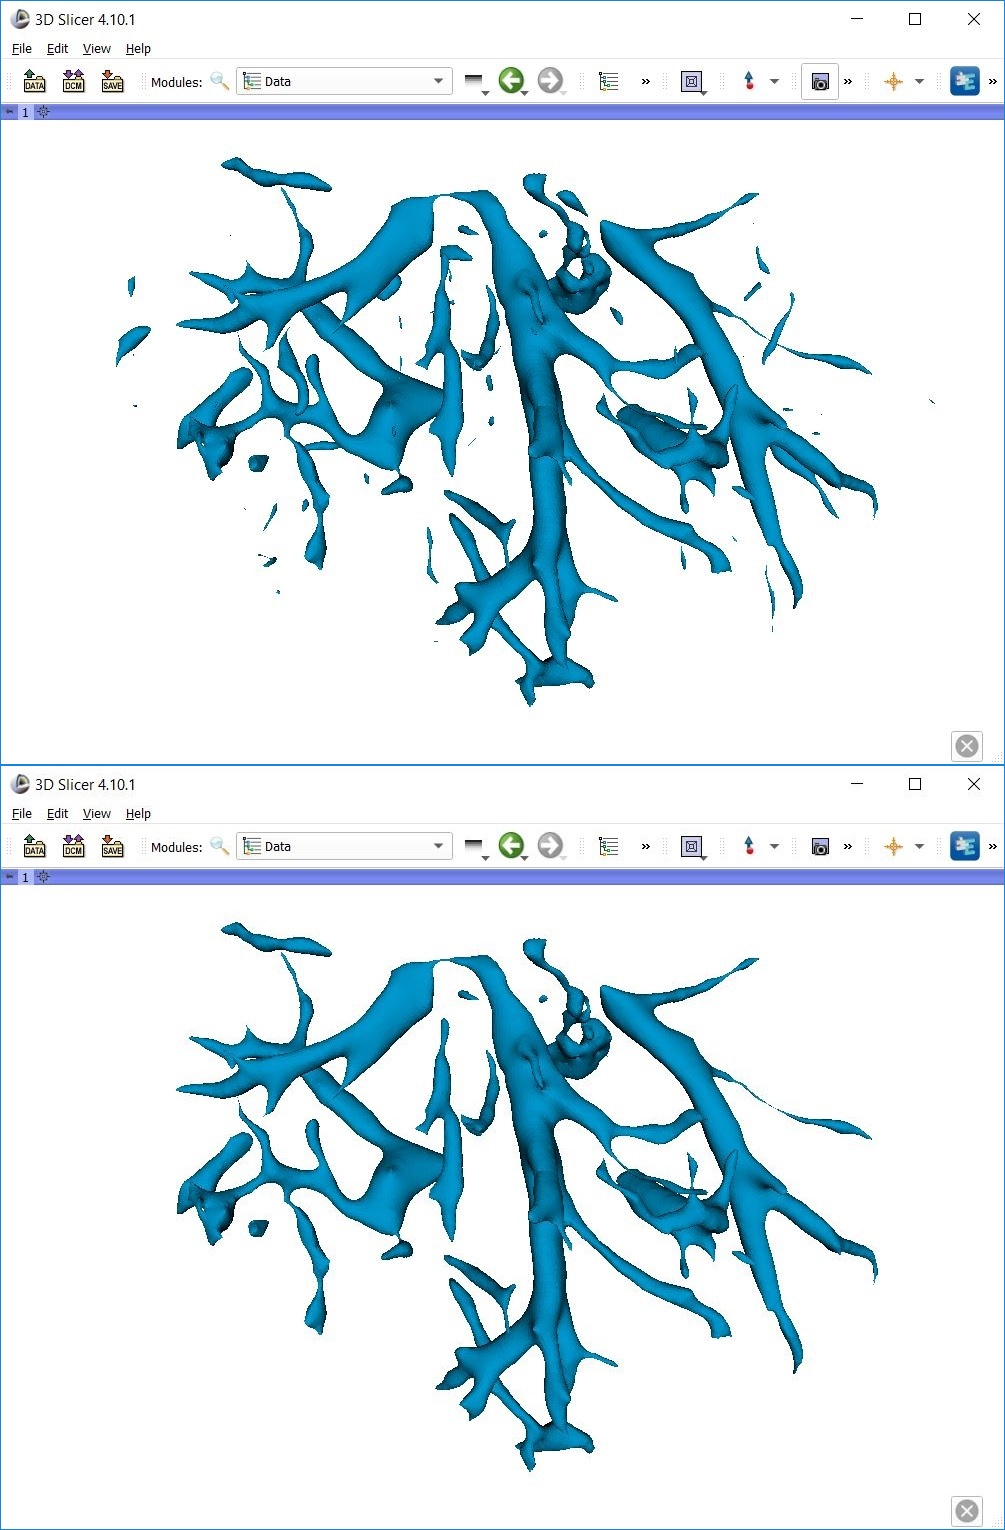
\includegraphics[width=\textwidth, height=.925\textheight]{figures/result_e2_best_prediction_post_processing}
% 		\caption[Kết quả hệ thống mạch máu của trường hợp tốt nhất trong thí nghiệm 2.]{Kết quả hệ thống mạch máu của trường hợp tốt nhất trong thí nghiệm 2 trước và sau hậu xử lý. Các thành phần nhỏ và rời rạc đã được loại bỏ.}
% 		\label{fig:result_e2_best_prediction_post_processing}
% 	\end{figure}
% 	\begin{figure}[h!]
% 		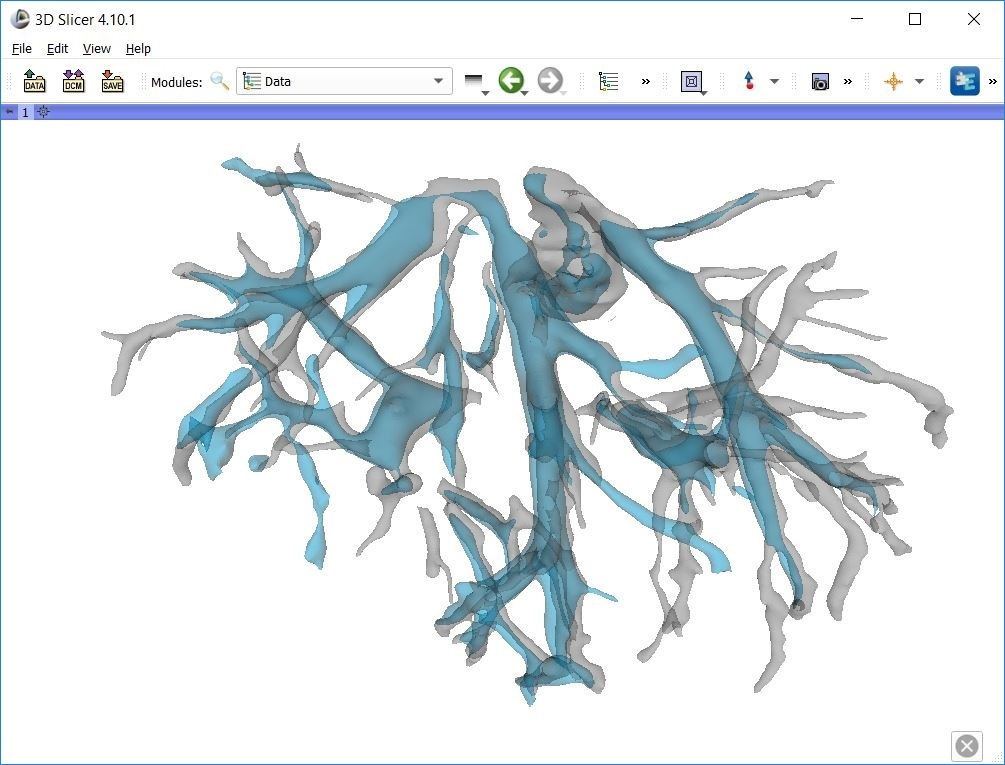
\includegraphics[width=\textwidth]{figures/result_e2_best_comparison}
% 		\caption[Kết quả hệ thống mạch máu của trường hợp tốt nhất trong thí nghiệm 2 và nhãn phân đoạn.]{Kết quả hệ thống mạch máu (màu xanh) của trường hợp tốt nhất trong thí nghiệm 2 khi so sánh với nhãn phân đoạn (màu xám). Hệ thống đã phân đoạn được các nhánh chính của mạch máu, tuy nhiên, còn rất nhiều nhánh mạch máu nhỏ hệ thống chưa phân đoạn được.}
% 		\label{fig:result_e2_best_comparison}
% 	\end{figure}
% 	\begin{figure}[h!]
% 		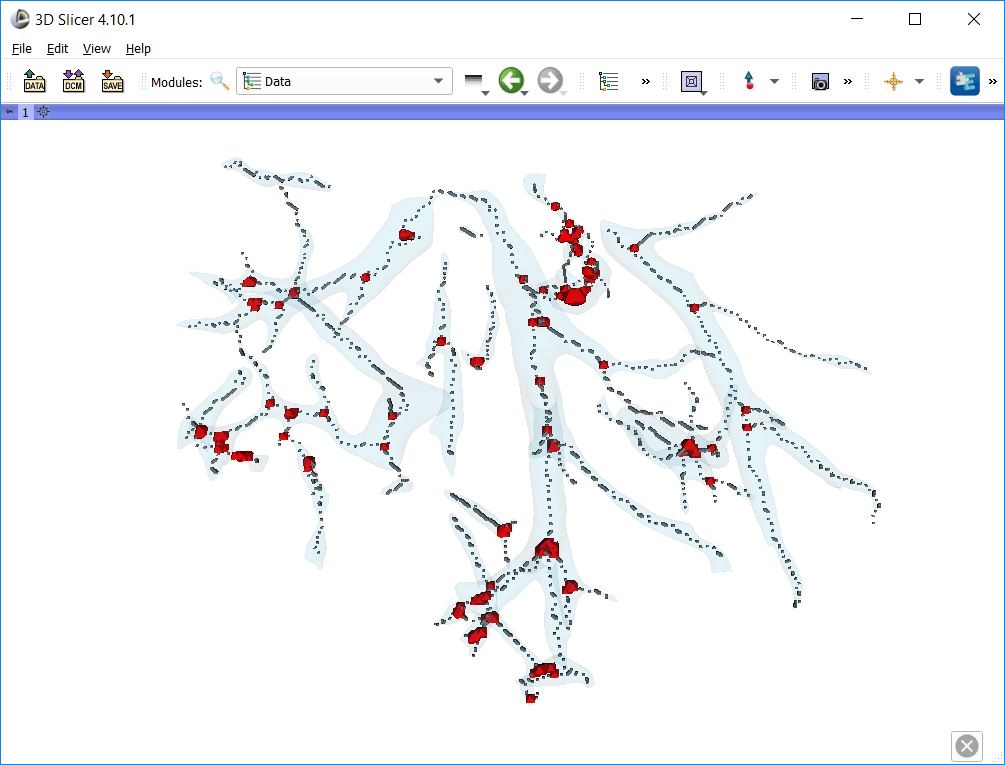
\includegraphics[width=\textwidth]{figures/result_e2_best_skeleton_branching_point}
% 		\caption[Kết quả tìm đường chính giữa và điểm phân nhánh của trường hợp tốt nhất trong thí nghiệm 2.]{Kết quả tìm đường chính giữa (đường màu xám) và điểm phân nhánh (màu đỏ) của trường hợp tốt nhất trong thí nghiệm 2. Hệ thống đã xác định được đường chính giữa và các điểm phân nhánh của mạch máu.}
% 		\label{fig:result_e2_best_skeleton_branching_point}
% 	\end{figure}


% 	\begin{figure}[h!]
% 		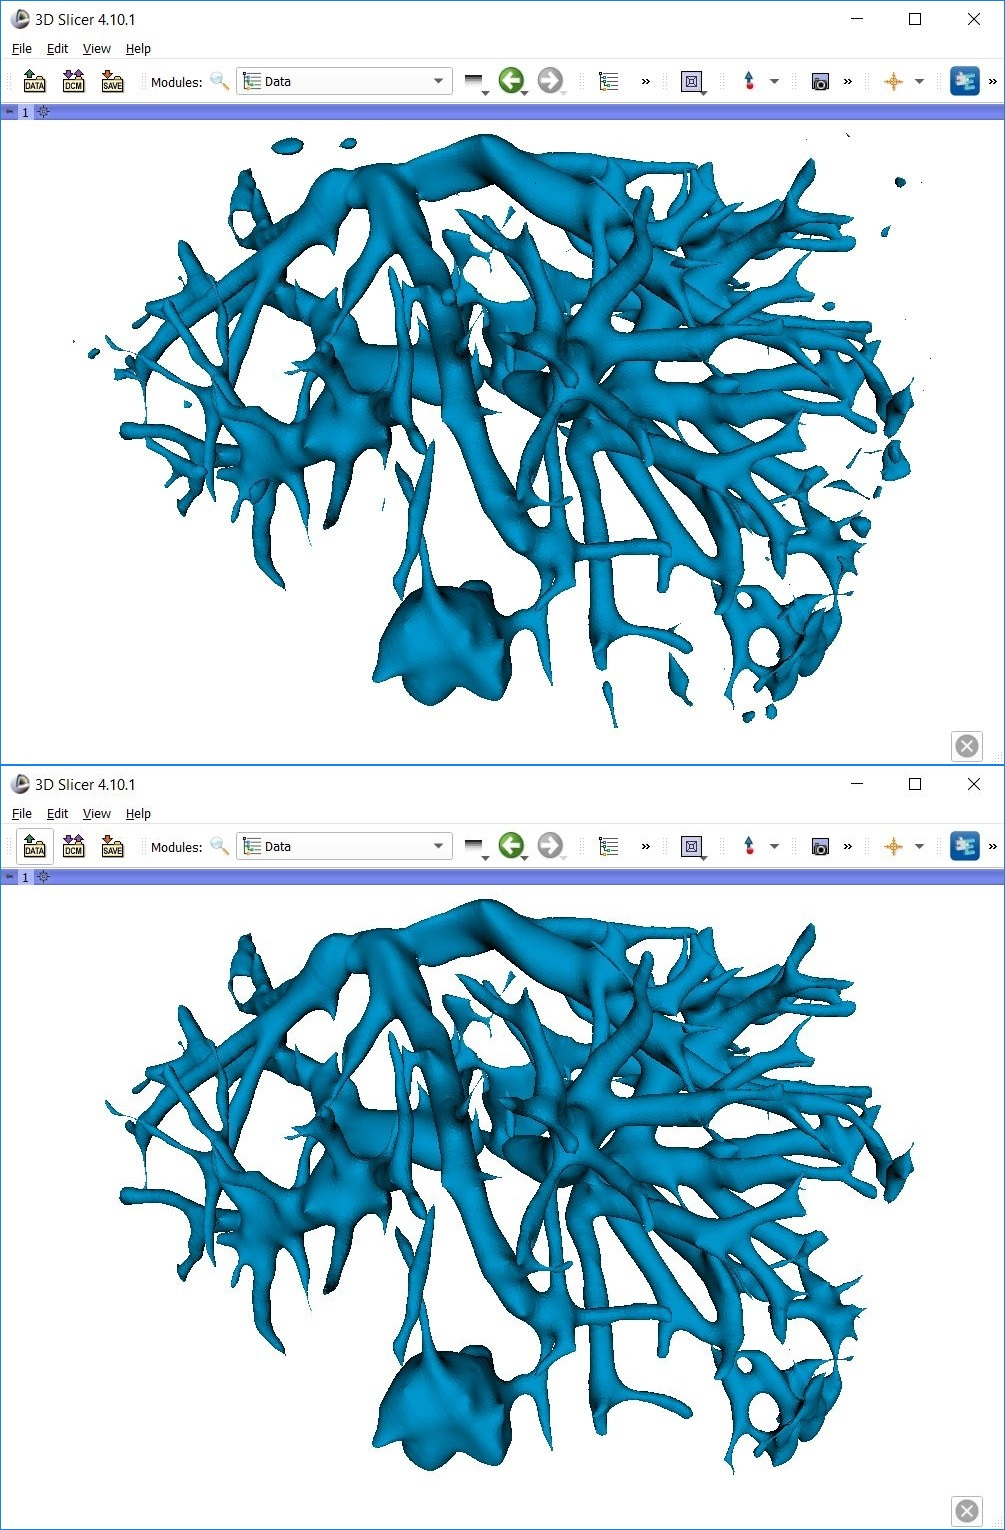
\includegraphics[width=\textwidth, height=0.925\textheight]{figures/result_e2_worst_prediction_post_processing}
% 		\caption[Kết quả hệ thống mạch máu của trường hợp xấu nhất trong thí nghiệm 2.]{Kết quả hệ thống mạch máu của trường hợp xấu nhất trong thí nghiệm 2 trước và sau hậu xử lý. Hệ thống phân đoạn mạch máu quá lớn, bước hậu xử lý không có nhiều hiệu quả.}
% 		\label{fig:result_e2_worst_prediction_post_processing}
% 	\end{figure}
% 	\begin{figure}[h!]
% 		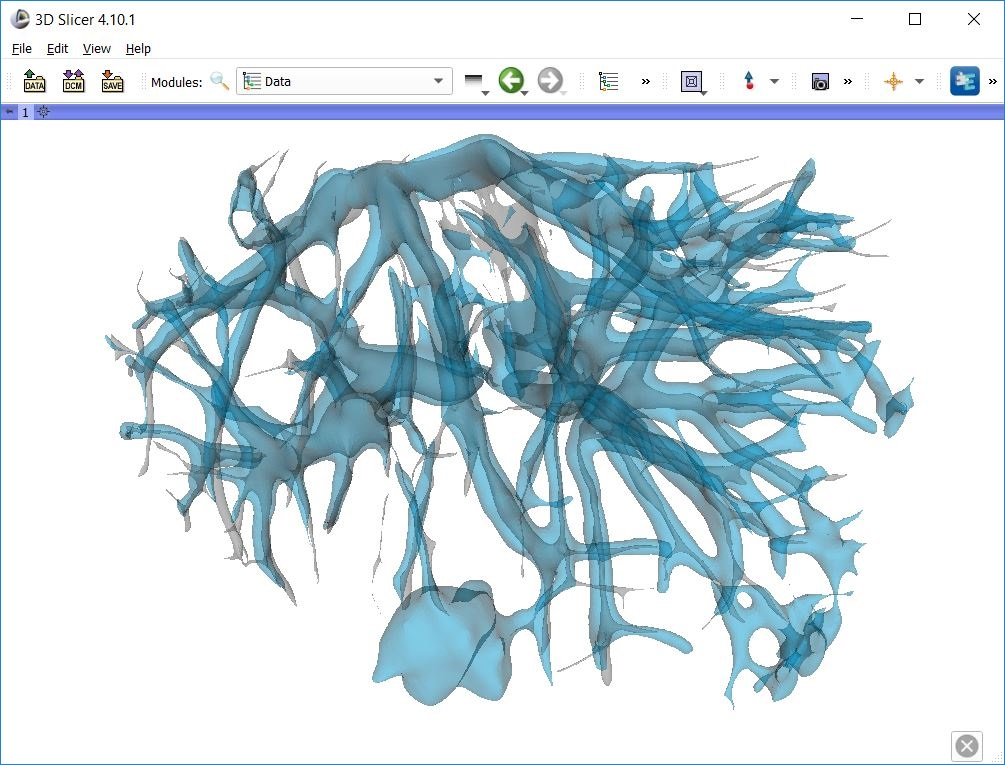
\includegraphics[width=\textwidth]{figures/result_e2_worst_comparison}
% 		\caption[Kết quả hệ thống mạch máu của trường hợp xấu nhất trong thí nghiệm 2 và nhãn phân đoạn.]{Kết quả hệ thống mạch máu (màu xanh) của trường hợp xấu nhất trong thí nghiệm 2 khi so sánh với nhãn phân đoạn (màu xám). Các mạch máu được phân đoạn lớn hơn rất nhiều so với thực tế. Ngoài ra, xuất hiện một khối phân đoạn sai rất lớn có thể là khối u.}
% 		\label{fig:result_e2_worst_comparison}
% 	\end{figure}
% 	\begin{figure}[h!]
% 		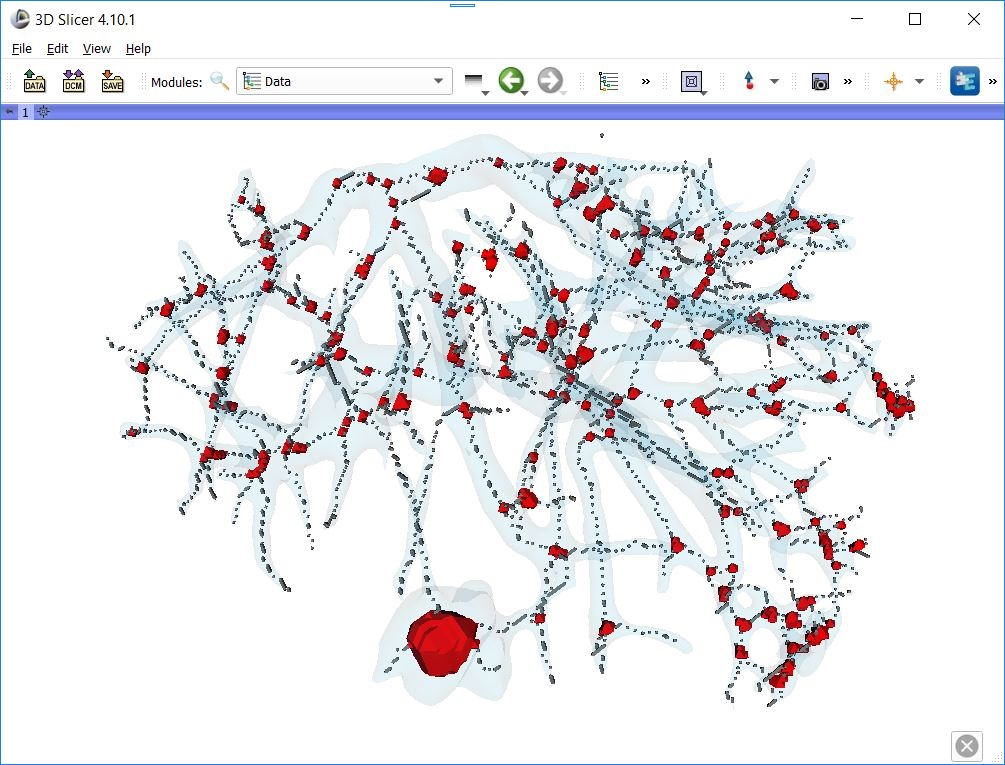
\includegraphics[width=\textwidth]{figures/result_e2_worst_skeleton_branching_point}
% 		\caption[Kết quả tìm đường chính giữa và điểm phân nhánh của trường hợp xấu nhất trong thí nghiệm 2.]{Kết quả tìm đường chính giữa (đường màu xám) và điểm phân nhánh (màu đỏ) của trường hợp xấu nhất trong thí nghiệm 2. Hệ thống đã xác định được đường chính giữa và các điểm phân nhánh của mạch máu. Tuy nhiên, xuất hiện rất nhiều điểm phân nhánh sai.}
% 		\label{fig:result_e2_worst_skeleton_branching_point}
% 	\end{figure}

% 	\begin{figure}[h!]
% 		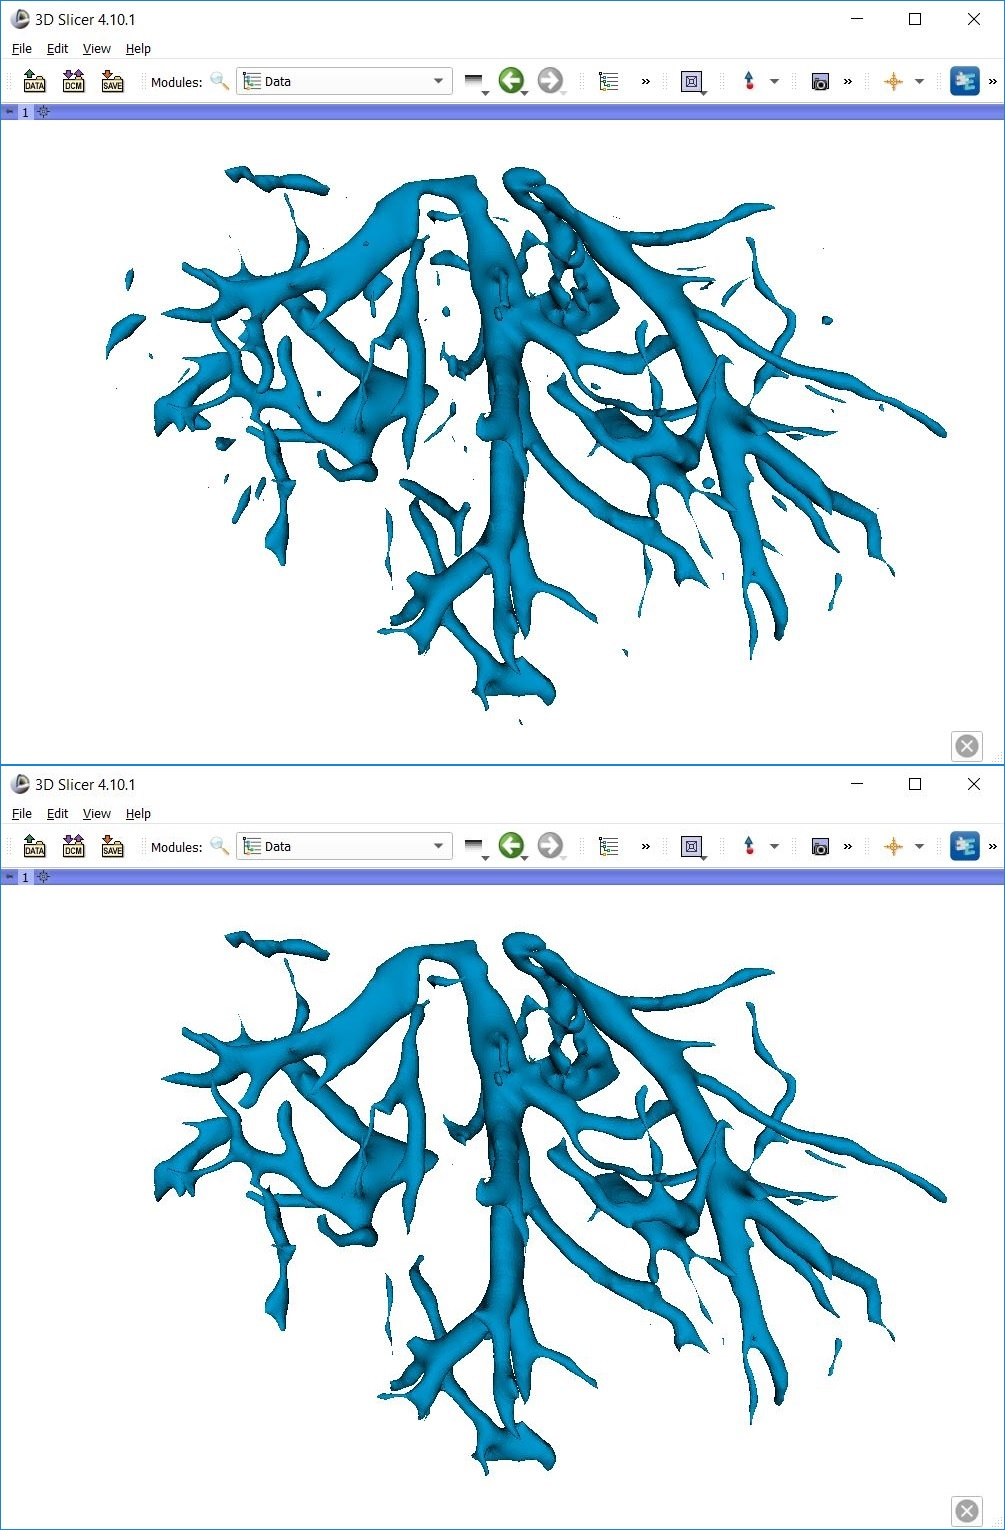
\includegraphics[width=\textwidth, height=0.925\textheight]{figures/result_e8_best_prediction_post_processing}
% 		\caption[Kết quả hệ thống mạch máu của trường hợp tốt nhất trong thí nghiệm 8.]{Kết quả hệ thống mạch máu của trường hợp tốt nhất trong thí nghiệm 8 trước và sau hậu xử lý. Các thành phần nhỏ và rời rạc hầu như đã được loại bỏ hoàn toàn.}
% 		\label{fig:result_e8_best_prediction_post_processing}
% 	\end{figure}
% 	\begin{figure}[h!]
% 		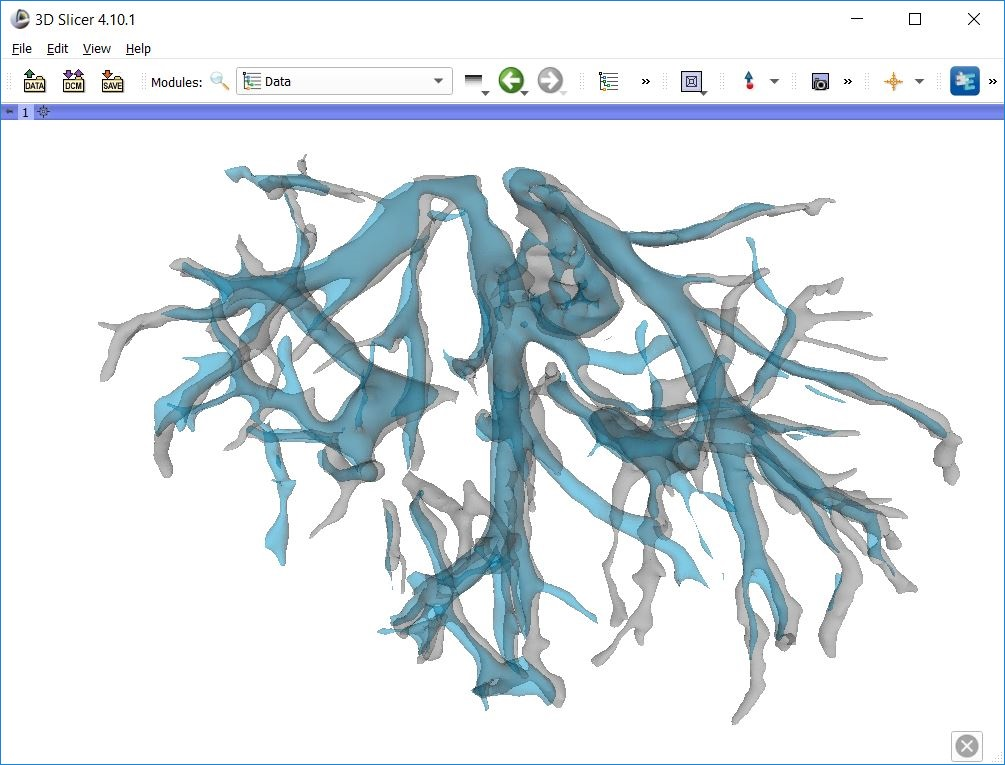
\includegraphics[width=\textwidth]{figures/result_e8_best_comparison}
% 		\caption[Kết quả hệ thống mạch máu của trường hợp tốt nhất trong thí nghiệm 8 và nhãn phân đoạn.]{Kết quả hệ thống mạch máu (màu xanh) của trường hợp tốt nhất trong thí nghiệm 8 khi so sánh với nhãn phân đoạn (màu xám). Kết quả phân đoạn khá sát với thực tế, chỉ một vài nhánh nhỏ chưa phân đoạn được.}
% 		\label{fig:result_e8_best_comparison}
% 	\end{figure}
% 	\begin{figure}[h!]
% 		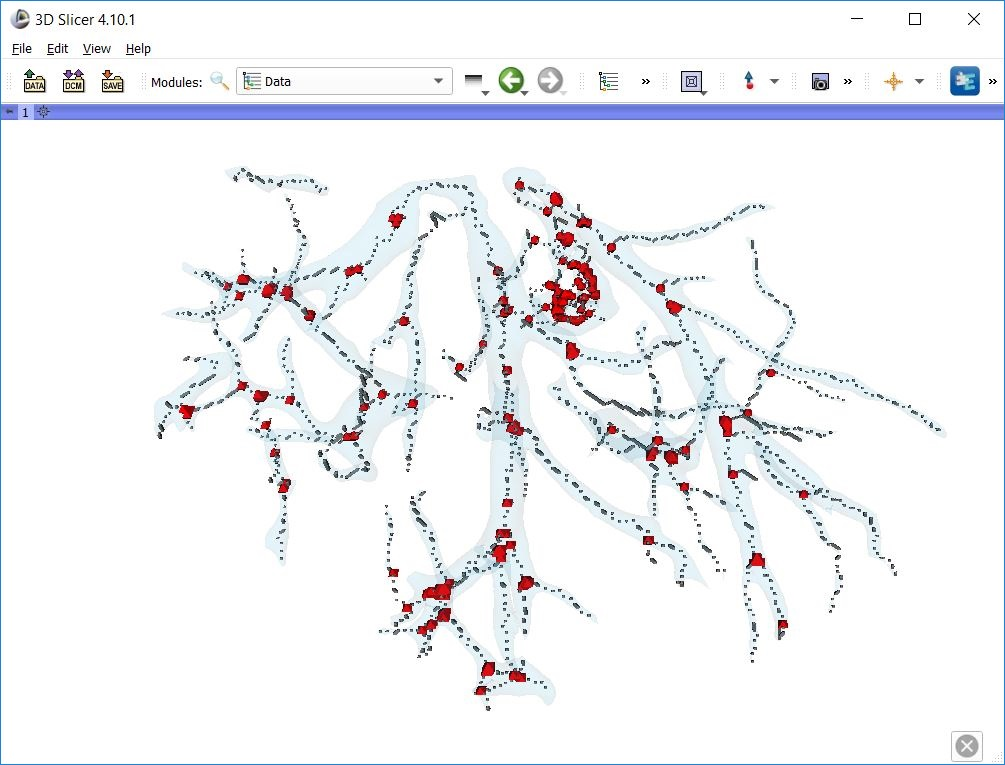
\includegraphics[width=\textwidth]{figures/result_e8_best_skeleton_branching_point}
% 		\caption[Kết quả tìm đường chính giữa và điểm phân nhánh của trường hợp tốt nhất trong thí nghiệm 8.]{Kết quả tìm đường chính giữa (đường màu xám) và điểm phân nhánh (màu đỏ) của trường hợp tốt nhất trong thí nghiệm 8. Hệ thống đã xác định được đường chính giữa và các điểm phân nhánh của mạch máu.}
% 		\label{fig:result_e8_best_skeleton_branching_point}
% 	\end{figure}
% 	\begin{figure}[h!]
% 		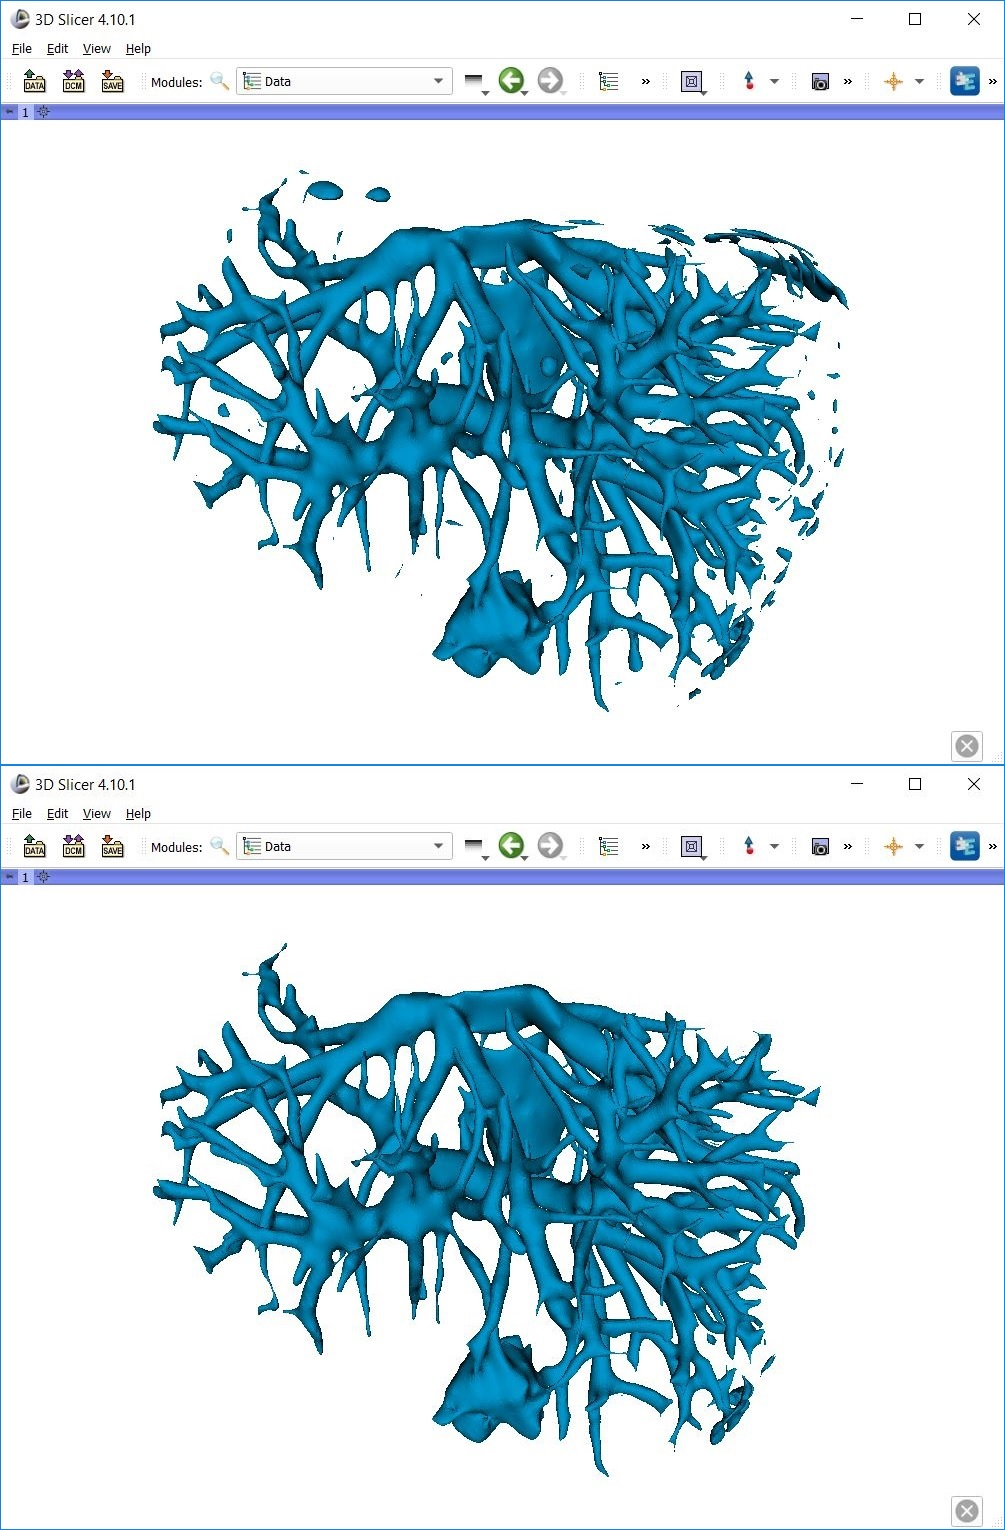
\includegraphics[width=\textwidth, height=0.925\textheight]{figures/result_e8_worst_prediction_post_processing}
% 		\caption[Kết quả hệ thống mạch máu của trường hợp xấu nhất trong thí nghiệm 8.]{Kết quả hệ thống mạch máu của trường hợp xấu nhất trong thí nghiệm 8 trước và sau hậu xử lý. Bước hậu xử lý đã loại bỏ đi rất nhiều vị trí dự đoán sai.}
% 		\label{fig:result_e8_worst_prediction_post_processing}
% 	\end{figure}
% 	\begin{figure}[h!]
% 		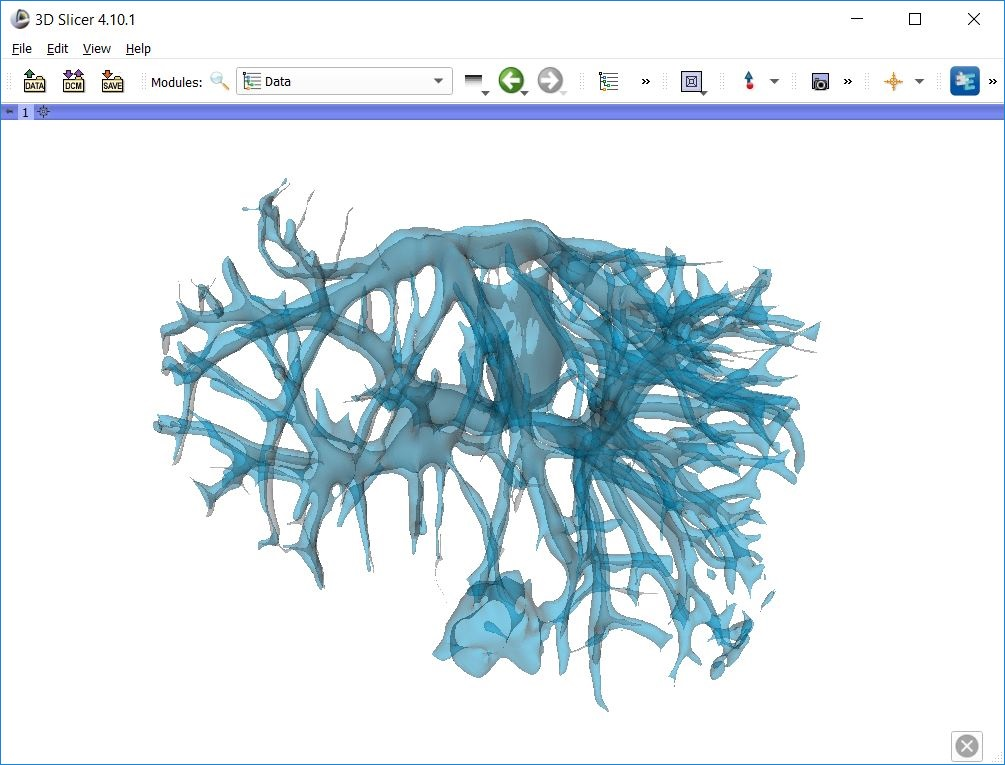
\includegraphics[width=\textwidth]{figures/result_e8_worst_comparison}
% 		\caption[Kết quả hệ thống mạch máu của trường hợp xấu nhất trong thí nghiệm 8 và nhãn phân đoạn.]{Kết quả hệ thống mạch máu (màu xanh) của trường hợp xấu nhất trong thí nghiệm 8 khi so sánh với nhãn phân đoạn (màu xám). Các mạch máu được phân đoạn lớn hơn rất nhiều so với thực tế. Ngoài ra, xuất hiện một khối phân đoạn sai rất lớn có thể là khối u.}
% 		\label{fig:result_e8_worst_comparison}
% 	\end{figure}
% 	\begin{figure}[h!]
% 		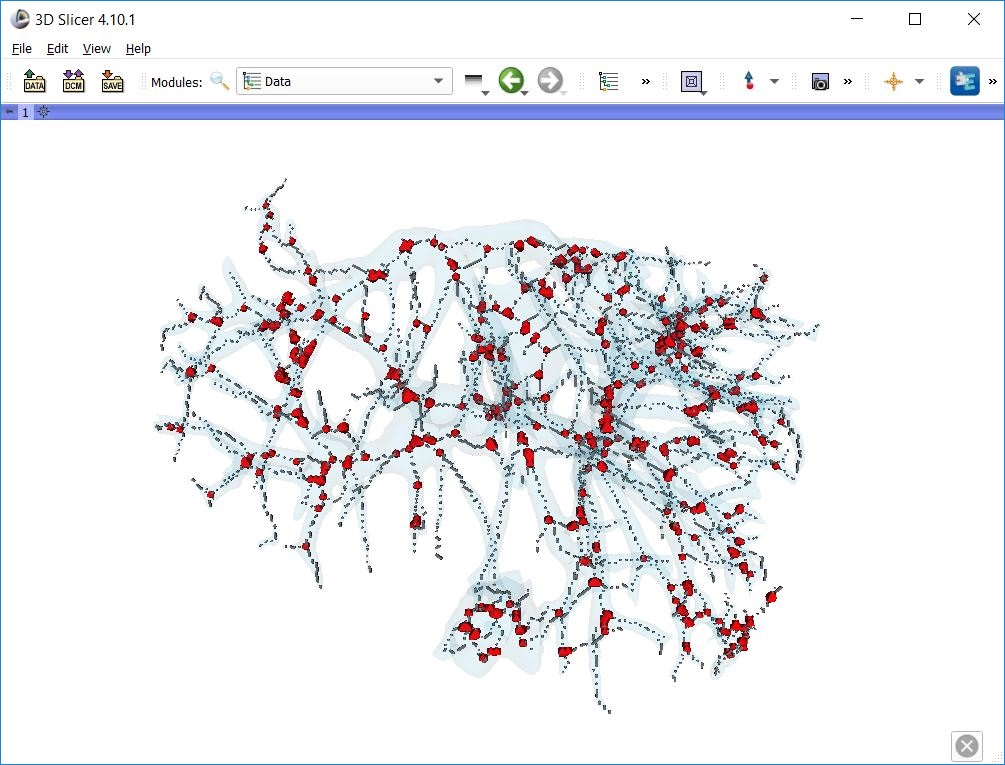
\includegraphics[width=\textwidth]{figures/result_e8_worst_skeleton_branching_point}
% 		\caption[Kết quả tìm đường chính giữa và điểm phân nhánh của trường hợp xấu nhất trong thí nghiệm 8.]{Kết quả tìm đường chính giữa (đường màu xám) và điểm phân nhánh (màu đỏ) của trường hợp xấu nhất trong thí nghiệm 8. Hệ thống đã xác định được đường chính giữa và các điểm phân nhánh của mạch máu. Tuy nhiên, xuất hiện rất nhiều đường chính giữa và điểm phân nhánh sai.}
% 		\label{fig:result_e8_worst_skeleton_branching_point}
% 	\end{figure}